\documentclass{beamer}

\usepackage{graphicx}

\title{Algorithmic Trading System: Group 03}
\author{George El Boustani, Nicholas Grasevski, Daniel Morton, Christopher Tin-Loi}
\date{\today}

\begin{document}

\begin{frame}
\titlepage
\end{frame}

\begin{frame}
\frametitle{Implemented requirements}
\begin{description}
  \item[F1] Reading a correctly formatted Sirca orders file
  \item[F2] Choosing an appropriate algorithmic trading strategy and setting its different parameters
  \item[F3] Generating algorithmic orders for 1 particular day
  \item[F4] Generating algorithmic trades for 1 particular day
  \item[F5] Evaluating algorithmic trades and providing feedback to user
  \item[F6] Generating a strategy performance report
  \item[F7] GUI functions to control use cases to load and execute an orders file
\end{description}
\end{frame}

\begin{frame}
\frametitle{Architecture}
\begin{figure}
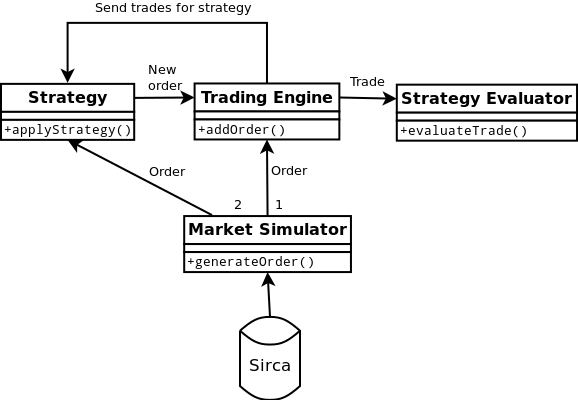
\includegraphics[width=0.8\linewidth]{architecture}
\end{figure}
\end{frame}

\begin{frame}
\frametitle{Advantages of our system}
\begin{description}
  \item[Fast] Leverages the performance of Python's parsing and number crunching libraries
  \item[Flexible] GUI, CLI and library provided, allowing for a variety of use cases
  \item[Customizable] User can write their own strategies/engines/evaluators as plugins
  \item[Usable] Simple and intuitive GUI
\end{description}
\end{frame}

\end{document}
